\documentclass[]{article}
\usepackage{lmodern}
\usepackage{amssymb,amsmath}
\usepackage{ifxetex,ifluatex}
\usepackage{fixltx2e} % provides \textsubscript
\ifnum 0\ifxetex 1\fi\ifluatex 1\fi=0 % if pdftex
  \usepackage[T1]{fontenc}
  \usepackage[utf8]{inputenc}
\else % if luatex or xelatex
  \ifxetex
    \usepackage{mathspec}
    \usepackage{xltxtra,xunicode}
  \else
    \usepackage{fontspec}
  \fi
  \defaultfontfeatures{Mapping=tex-text,Scale=MatchLowercase}
  \newcommand{\euro}{€}
\fi
% use upquote if available, for straight quotes in verbatim environments
\IfFileExists{upquote.sty}{\usepackage{upquote}}{}
% use microtype if available
\IfFileExists{microtype.sty}{%
\usepackage{microtype}
\UseMicrotypeSet[protrusion]{basicmath} % disable protrusion for tt fonts
}{}
\usepackage[margin=1in]{geometry}
\ifxetex
  \usepackage[setpagesize=false, % page size defined by xetex
              unicode=false, % unicode breaks when used with xetex
              xetex]{hyperref}
\else
  \usepackage[unicode=true]{hyperref}
\fi
\hypersetup{breaklinks=true,
            bookmarks=true,
            pdfauthor={Fauzy bin Che Yayah},
            pdftitle={Text Data Processing Techniques on Trouble Ticket for Enhancing Resolution Knowledge},
            colorlinks=true,
            citecolor=blue,
            urlcolor=blue,
            linkcolor=magenta,
            pdfborder={0 0 0}}
\urlstyle{same}  % don't use monospace font for urls
\usepackage{natbib}
\bibliographystyle{plainnat}
\usepackage{longtable,booktabs}
\usepackage{graphicx,grffile}
\makeatletter
\def\maxwidth{\ifdim\Gin@nat@width>\linewidth\linewidth\else\Gin@nat@width\fi}
\def\maxheight{\ifdim\Gin@nat@height>\textheight\textheight\else\Gin@nat@height\fi}
\makeatother
% Scale images if necessary, so that they will not overflow the page
% margins by default, and it is still possible to overwrite the defaults
% using explicit options in \includegraphics[width, height, ...]{}
\setkeys{Gin}{width=\maxwidth,height=\maxheight,keepaspectratio}
\setlength{\parindent}{0pt}
\setlength{\parskip}{6pt plus 2pt minus 1pt}
\setlength{\emergencystretch}{3em}  % prevent overfull lines
\providecommand{\tightlist}{%
  \setlength{\itemsep}{0pt}\setlength{\parskip}{0pt}}
\setcounter{secnumdepth}{5}

%%% Use protect on footnotes to avoid problems with footnotes in titles
\let\rmarkdownfootnote\footnote%
\def\footnote{\protect\rmarkdownfootnote}

%%% Change title format to be more compact
\usepackage{titling}

% Create subtitle command for use in maketitle
\newcommand{\subtitle}[1]{
  \posttitle{
    \begin{center}\large#1\end{center}
    }
}

\setlength{\droptitle}{-2em}
  \title{Text Data Processing Techniques on Trouble Ticket for Enhancing
Resolution Knowledge}
  \pretitle{\vspace{\droptitle}\centering\huge}
  \posttitle{\par}
  \author{Fauzy bin Che Yayah}
  \preauthor{\centering\large\emph}
  \postauthor{\par}
  \predate{\centering\large\emph}
  \postdate{\par}
  \date{November 21, 2015}


% Redefines (sub)paragraphs to behave more like sections
\ifx\paragraph\undefined\else
\let\oldparagraph\paragraph
\renewcommand{\paragraph}[1]{\oldparagraph{#1}\mbox{}}
\fi
\ifx\subparagraph\undefined\else
\let\oldsubparagraph\subparagraph
\renewcommand{\subparagraph}[1]{\oldsubparagraph{#1}\mbox{}}
\fi

\begin{document}
\maketitle

{
\hypersetup{linkcolor=black}
\setcounter{tocdepth}{2}
\tableofcontents
}
\pagebreak

\emph{Abstract -Trouble ticket system is always includes very rich data,
but how to data-mining from is very challenging task.In this paper , we
applied the technique of data processing for the ease for the next stage
of classification and prediction.On the other hand , we applied the new
techniques of data mining by combining with the Bigdata elements for
faster and achievable results.We realize that the combination of this
techniques will provide luxuriant decision information for any
organization and management.It also can become a fulfillment the field
of data mining}

\section{Keywords}\label{keywords}

Data mining; data processing ; hadoop ; tickets data ; unstructured text
processing

\section{Introduction}\label{introduction}

The trouble ticket system for telecommunication industries produced
several thousand of records everyday. These records provide rich,
accurate and complete for the system diagnostics and enhancing the
customer experience by solving the problems. The live records stored
inside the database of all levels of servers and replicated into the
Enterprise Data Warehouse (EDWH) for data staging and shared among the
departments via the credential and permission for different points of
usage or use case. The data are coordinated and conserved for at least
for five years minimum, which is enough for the analytics and data
discovery purpose. The remaining more than five years of data will not
be discarded and the archiving process will be applied for future
reference. Because of the EDWH is optimized for storage, any heavily
queries for analytics purpose in the system is not recommended which
this activity will jeopardize the overall system performance.

\section{Related work}\label{related-work}

\subsection{Introduction of TTS}\label{introduction-of-tts}

The trouble ticket system is considered as an assistant software which
implements the Decision Support System (DSS) that manage and maintain
lists of issues recorded by the customer support call center. The system
contains a knowledge based containing the vital information for each
subscribed customer, common resolution for most of the problems, and
other such data. The ticket is the details of particular problem which
contains the ticket status and other relevant data.

\begin{figure}[htbp]
\centering
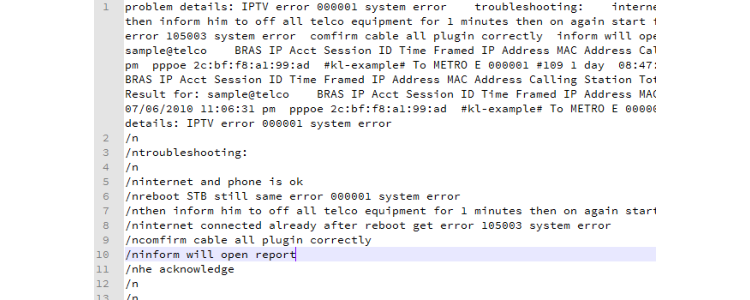
\includegraphics{Journal1_files/figure-latex/unnamed-chunk-4-1.pdf}
\caption{Trouble ticket system with predictive analytics framework}
\end{figure}

\subsection{Basic structure of trouble ticket
data}\label{basic-structure-of-trouble-ticket-data}

The dataset of customer trouble ticket mainly comes from the trouble
ticket system (TTS). The data set, then distributed into different
levels of staging servers and other type database system at different
levels of credential. The table below is a list of some fields from the
trouble ticket table which mapped from the CTTS database :-

\begin{longtable}[c]{@{}lll@{}}
\toprule
Column Name & Column Type & Notes\tabularnewline
\midrule
\endhead
id & String & Generated ID by the system\tabularnewline
created\_dt & DateTime & Date of the trouble ticket
creation\tabularnewline
closed\_dt & DateTime & Date of the trouble ticket closed\tabularnewline
symp\_err & String & Symptom error detected\tabularnewline
cause\_cat & String & Category Code define by the system\tabularnewline
cause\_code & String & Cause Code define by the system\tabularnewline
res\_code & String & Resolution Code define\tabularnewline
desc & Text & Detail textual information such as\tabularnewline
& & customer information, session status,\tabularnewline
& & system status, network status , etc.\tabularnewline
& & Cause Code define by the system\tabularnewline
acc\_name & String & Name of the customer\tabularnewline
acc\_num & String & Account number of the customer\tabularnewline
package & String & Main package subscribed by the
customers\tabularnewline
zone & String & Product affected zone\tabularnewline
\ldots{}. & \ldots{}. & \ldots{}.\tabularnewline
\bottomrule
\end{longtable}

In summary , this table below is the sample of TTS records :-

\begin{longtable}[c]{@{}lll@{}}
\toprule
Column Type & Example & Field Name\tabularnewline
\midrule
\endhead
Integer & {[}1001{]} , {[}1002{]} , {[}1003{]} & ID\tabularnewline
DateTime & {[}2012-09-05 19:39:01.0{]},{[}2012-09-05 19:45:39.0{]} &
created\_dt\tabularnewline
Text & \emph{``Troubleshooting Step: -check outages -check account
status''} & desc\tabularnewline
String & {[}Performance{]} , {[}Failure{]}, {[}Open{]}, {[}Closed{]} &
symp\_err\tabularnewline
\ldots{}. & \ldots{}. & \ldots{}.\tabularnewline
\bottomrule
\end{longtable}

We identify the structure inside the TTS (\emph{desc}) contains a free
text form inside the description field. This is in need for search and
analyze inside it. The data need to transform into something that can
have a better understanding and more effective representation. A TTS
description is fill-up by capturing from the customer call center or by
the technician from the two major sources such as email and subsequent
call from the customer.Thus, most of the data is not explicitly
structured, it is also highly noisy (e.g, inconsistent formatting) and
also very heterogenous (e.g., multiple language, such as Bahasa Melayu
or English, system generated data, specific telecommunication term ,
abbreviation , acronyms and jargons),making it hard to analyze and
search information from the raw data. We introduced an approach for
automatically search for specific knowledge or topics from the
collection of the free from text section (desc) inside the TTS.

\pagebreak

\section{Techniques}\label{techniques}

Our elegant methodology automatically structuring free-from heterogenous
textual data helps to identify the structural pattern specific pattern
known to the call center of technician which helps them to speed up the
tedious work manually searching and understanding the relevant data
inside it. Below is the workflow for this methodology :-

\begin{itemize}
\tightlist
\item
  Acquiring with basic filtering TTS dataset from EDWH into Hadoop using
  Sqoop
\item
  Applying index number for TTS dataset inside Hive
\item
  Second filtering of TTS dataset
\item
  Create a Document Term Matrix (DTM)
\item
  Sparse Terms Removal
\item
  Vectorization of TTS (VTTS)
\end{itemize}

\subsection{Acquiring with basic filtering TTS dataset from EDWH into
Hadoop using
Sqoop}\label{acquiring-with-basic-filtering-tts-dataset-from-edwh-into-hadoop-using-sqoop}

To acquire TTS dataset from the EDWH we need special operation using
\emph{Sqoop} components inside Hadoop into Hive compatible format.
Hadoop is an open-source software framework for storing data and running
applications on clusters of commodity hardware. Hive is a data warehouse
infrastructure built on top of Hadoop for providing data summarization,
query, and analysis.Sqoop is a tool designed to transfer data between
Hadoop and relational database servers.

\begin{figure}[htbp]
\centering
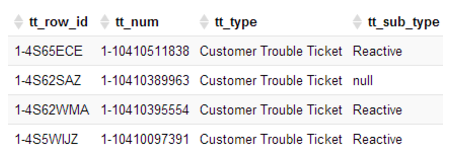
\includegraphics{Journal1_files/figure-latex/unnamed-chunk-6-1.pdf}
\caption{Hadoop - Sqoop - Hive Operation}
\end{figure}

Sqoop basic syntax for importing dataset from TTS as follows :-

\begin{verbatim}
sqoop import --connect jdbc:[rdbms driver]:@[ip_address]:[port]/[db_name] 
--username [username] --password [password]  --target-dir [temp_target]  --verbose 
-e "select [field[1:n],REGEXP_REPLACE([desc_field_name],
'[^a-zA-Z0-9\\:\\@\\/\\#\\-]', ' ') " --m 1 --hive-table 
[dbname_in_hdfs][tablename_inhdfs] --hive-import
--append --fields-terminated-by '\001'  
--lines-terminated-by '\n' --hive-delims-replacement '';
\end{verbatim}

\pagebreak

Description of the syntax above as follows :-

\begin{longtable}[c]{@{}ll@{}}
\toprule
Syntax & Description\tabularnewline
\midrule
\endhead
sqoop import & Import a table from a database to HDFS\tabularnewline
--connect jdbc:{[}rdbms driver{]} & Specify JDBC connect
string\tabularnewline
{[}ip\_address{]}:{[}port{]}/{[}db\_name{]} & Provides ip address , port
no and rdbms database name\tabularnewline
--username {[}username{]} & Provides the username\tabularnewline
--password {[}password{]} & Provides the password\tabularnewline
--target-dir {[}temp\_target{]} & Specify the target path for the output
of the merge job\tabularnewline
--verbose & Print information while execute\tabularnewline
-e & specified query statement\tabularnewline
\emph{select} & statement returns a result set of records from one or
more tables\tabularnewline
{[}field{[}1:n{]} &\tabularnewline
REGEXP\_REPLACE({[}desc\_field\_name{]},) & search a string for a
regular expression pattern\tabularnewline
`{[}\^{}a-zA-Z0-9\textbackslash{}\textbackslash{}:\textbackslash{}\textbackslash{}@\textbackslash{}\textbackslash{}/\textbackslash{}\textbackslash{}\#\textbackslash{}\textbackslash{}-{]}',
`') & remove all special characters and numbers\tabularnewline
{[}-m 1{]} & Use n map tasks to import in parallel\tabularnewline
{[}--hive-table & Sets the table name to use when importing to
Hive\tabularnewline
{[}{[}dbname\_in\_hdfs{]} & Sets the db name in Hive/HDFS\tabularnewline
{[}tablename\_inhdfs{]} & Sets the db name in Hive/HDFS\tabularnewline
--hive-import & Import tables into Hive format\tabularnewline
--append & Append data to an existing dataset in HDFS\tabularnewline
--fields-terminated-by `\textbackslash{}001' & Sets the field separator
character\tabularnewline
--lines-terminated-by `\textbackslash{}n' & Sets the end-of-line
character\tabularnewline
--hive-delims-replacement '' & Replace delimiter from string fields with
user defined string\tabularnewline
\bottomrule
\end{longtable}

To make, it is safe to resides into the Hive table, any special
character set by \texttt{REGEXP\_REPLACE} found during acquiring the
dataset will be replaced with default delimiter \texttt{NULL} or empty
char. this can be achieved by applying the
\texttt{-\/-hive-delims-replacement\ \textquotesingle{}\textquotesingle{}}
and \texttt{REGEXP\_REPLACE}
\texttt{{[}\^{}a-zA-Z0-9\textbackslash{}\textbackslash{}:\textbackslash{}\textbackslash{}@\textbackslash{}\textbackslash{}/\textbackslash{}\textbackslash{}\#\textbackslash{}\textbackslash{}-{]}}
inside the command line while sqoop is executed. The comparison images
below shows the clean up results before and after applying the regular
expression filtering :-

\begin{figure}[htbp]
\centering
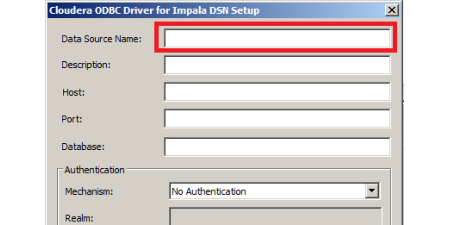
\includegraphics{Journal1_files/figure-latex/unnamed-chunk-8-1.pdf}
\caption{Original - (desc) field text}
\end{figure}

\begin{figure}[htbp]
\centering

\includegraphics{Journal1_files/figure-latex/unnamed-chunk-9-1.pdf}
\caption{Filtered - (desc) structure after applying REGEXP\_REPLACE
during \texttt{Sqoop} operation}
\end{figure}

\subsection{Applying index number for TTS dataset inside
Hive}\label{applying-index-number-for-tts-dataset-inside-hive}

Basic default Hive dataset doesn't have any \texttt{autonumber} data
type. The \texttt{autonumber} is very useful for primary key operation
or for filter the records. We applied the the autonumber to the TTS
dataset after the Sqoop operation finished. Because of the dataset which
resides inside Hadoop is in Hive format , we need to use external jar
file which is \texttt{hive-contrib-0.12.0-cdh5.1.2.jar} to create
autonumber for the entire records. The jar file can be called by
creating custom function as follows :-

\begin{verbatim}
drop function IF EXISTS row_sequence(); 
create function IF NOT EXISTS row_sequence() 
returns BIGINT location 'lib/hive-contrib-0.12.0-cdh5.1.2.jar'
symbol='org.apache.hadoop.hive.contrib.udf.UDFRowSequence';
\end{verbatim}

The rules applying the autonumber to the TTS dataset are to set by
limits command inside the Hive-SQL. This is to ensure the dataset
creation is reduced into single file inside the HDFS. Without the limit
statement the Hive dataset files is chunked into the multiple split and
the auto number sequence is set in 0 for each split or
\texttt{single\ reducer}. This will cause the each records autonumber or
it will be redundant. The Hive-SQL` command for this operation cab be
achived by :-

\begin{verbatim}
drop table IF EXISTS tts_stage1; 
create table IF NOT EXISTS tts_stage1 as select row_sequence() as id , 
* from [tts_table] limit 10000;
\end{verbatim}

\begin{longtable}[c]{@{}ll@{}}
\toprule
SQL-Hive & Description\tabularnewline
\midrule
\endhead
\texttt{drop\ table\ IF\ EXISTS\ tts\_stage1;} & Create table statement
if exist\tabularnewline
\texttt{create\ table\ IF\ NOT\ EXISTS\ tts\_stage1} & Create table and
add autonumber as the first field\tabularnewline
\texttt{as\ select\ row\_sequence()\ as\ id\ ,} & before the TTS
fields\tabularnewline
\texttt{*\ from\ {[}tts\_table{]}\ limit\ 10000;} & Select all the
fields from original TTS and limits for
\texttt{single\ reducer}\tabularnewline
\bottomrule
\end{longtable}

\begin{figure}[htbp]
\centering

\includegraphics{Journal1_files/figure-latex/unnamed-chunk-10-1.pdf}
\caption{Initial Hive TTS Dataset after Sqoop operation}
\end{figure}

\begin{figure}[htbp]
\centering
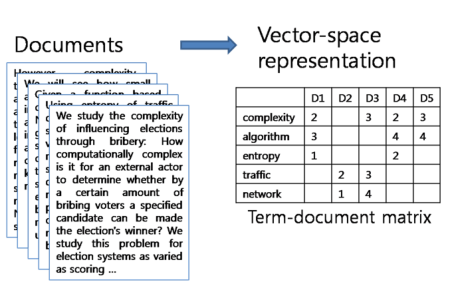
\includegraphics{Journal1_files/figure-latex/unnamed-chunk-11-1.pdf}
\caption{Posterior Hive TTS Dataset after applying Hive-SQL}
\end{figure}

\pagebreak

\subsection{Second filtering of TTS
dataset}\label{second-filtering-of-tts-dataset}

Since the dataset now are filled by autonumber \texttt{id}, now the
record can be filtered by the \texttt{id} range . Tools such as RStudio
which implements the R language statistical is used in this process.
RStudio is capable to connect to various datasources including Hive. In
this section , Open Database Connectivity(ODBC) for Hive need to be
installed and configured. ODBC for Hive can be downloaded from the
Cloudera website
(\url{http://www.cloudera.com/content/www/en-us/downloads/connectors/hive/odbc/2-5-12.html}).

\begin{figure}[htbp]
\centering
\includegraphics{Journal1_files/figure-latex/unnamed-chunk-13-1.pdf}
\caption{Hive ODBC Datasource Administrator}
\end{figure}

Set the ODBC data source name \emph{{[}dsn\_name{]}} , the host address
, the port number (default for \emph{Impala} is 21050 ; \emph{Hive} is
10000 ) , and the database name \emph{{[}db\_name{]}}. After that , test
the ODBC connection.

After the ODBC System DSN name have been set , use RStudio create new
\texttt{RScript} and implements the R code below for connnecting to Hive
ODBC via RODBC package. Package RODBC implements ODBC database
connectivity.
(\url{https://cran.r-project.org/web/packages/RODBC/vignettes/RODBC.pdf}).The
Rstudio can be downloaded from the Rstudio website.
(\url{https://www.rstudio.com/products/rstudio/download/}).

\begin{itemize}
\item
  Sample RScript to implements RODBC as follows :-

\begin{verbatim}
library(RODBC)  
conn <- odbcConnect(dsn="[dsn_name]", uid="[username]", pwd="[username]") #
queryResult <- sqlQuery(conn, "select desc from [db_name].[hive_table_with_id]
where id > 0 and id <= 10000 ")
odbcClose(conn)
\end{verbatim}
\end{itemize}

\begin{longtable}[c]{@{}ll@{}}
\toprule
R Script & Description\tabularnewline
\midrule
\endhead
\texttt{library(RODBC)} & load the RODBC instance
components\tabularnewline
\texttt{conn\ \textless{}-\ odbcConnect(dsn="{[}dsn\_name{]}"),} & Set
the DSN name\tabularnewline
\texttt{uid="{[}username{]}",\ pwd="{[}username{]}"} & set username and
password\tabularnewline
\texttt{sqlQuery(conn,\ "select\ desc\ from\ {[}hive\_table\_with\_id{]}"}
& Hive-SQL to filter the records\tabularnewline
\texttt{"where\ id\ \textgreater{}\ 0\ and\ id\ \textless{}=\ 10000"} &
Condition to select the records\tabularnewline
\texttt{odbcClose(conn)} & Cleans up and frees resources\tabularnewline
\bottomrule
\end{longtable}

Five stages of data filteration need to be applied to clean up
description text from the TTS information

\begin{longtable}[c]{@{}lll@{}}
\toprule
\# & Description & R Script with Regular Expression
filter\tabularnewline
\midrule
\endhead
1 & Lowercase all the charactors &
\texttt{df\_desc\ \textless{}-\ as.data.frame(tolower(df\_desc\$review))}\tabularnewline
2 & Remove all the numbers &
\texttt{df\_desc\ \textless{}-as.data.frame}\tabularnewline
& &
\texttt{(sapply(df\_desc,gsub,pattern="{[}{[}:digit:{]}{]}",replacement=""))}\tabularnewline
3 & Remove all the punctuation &
\texttt{df\_desc\textless{}-as.data.frame}\tabularnewline
& and symbols &
\texttt{(sapply(df\_desc,gsub,pattern="{[}{[}:punct:{]}{]}",replacement=""))}\tabularnewline
4 & Trim the unnecessary spaces &
\texttt{df\_desc\ \textless{}-as.data.frame}\tabularnewline
& &
\texttt{(sapply(df\_desc,gsub,pattern="@\textbackslash{}\textbackslash{}w+",replacement=""))}\tabularnewline
5 & Trimming the whitespace &
\texttt{df\_desc\ \textless{}-as.data.frame}\tabularnewline
& &
\texttt{(sapply(df\_desc,gsub,pattern="\^{}\textbackslash{}\textbackslash{}s+\textbar{}\textbackslash{}\textbackslash{}s+\$",replacement=""))}\tabularnewline
\bottomrule
\end{longtable}

The image below shows state of text description before applying the
regular expression by the RScript. The description text contains
irrelevant character types like numbers , special symbols , spaces ,
etc.

\begin{figure}[htbp]
\centering
\includegraphics{Journal1_files/figure-latex/unnamed-chunk-14-1.pdf}
\caption{description text on before filteration}
\end{figure}

After appying the five steps of filteration , now the text description
is suitable or the next stage of transformation which is Document Term
Matrix (DTM) . DTM is a mathematical matrix that describes the frequency
of terms that occur in a collection of documents. In this case the DTM
will tied to each of the TTS records.

\begin{figure}[htbp]
\centering
\includegraphics{Journal1_files/figure-latex/unnamed-chunk-15-1.pdf}
\caption{description text on after filteration}
\end{figure}

\subsection{Create a Document Term Matrix
(DTM)}\label{create-a-document-term-matrix-dtm}

Document Term Matrix (DTM) is a matrix based dataset which describes the
frequency of terms that occur inside collection of dataset especially
the text based types. The DTM was spesifically designed to have rows and
columns. Rows is correspond as related unique rows records
(\emph{documents}) and columns as the unique terms which exist inside
the selective column dataset.

\begin{figure}

{\centering \includegraphics{Journal1_files/figure-latex/unnamed-chunk-16-1} 

}

\caption{Document Term Matrix}\label{fig:unnamed-chunk-16}
\end{figure}

\pagebreak

The RScript below implements the Document Term Matrix function :-

\begin{verbatim}
      mach_corpus = Corpus(VectorSource(df_review$review))
      tdm = TermDocumentMatrix(mach_corpus,control = list(removePunctuation = TRUE,
      stopwords = c(stopwords("english")),
      removeNumbers = TRUE, tolower = TRUE))
      m <- as.matrix(tdm)
\end{verbatim}

The description of R Script as follows :-

\begin{longtable}[c]{@{}ll@{}}
\toprule
R Script & Description\tabularnewline
\midrule
\endhead
\texttt{Corpus(VectorSource(df\_review\$review))} & Representing and
computing on \texttt{corpora}.\tabularnewline
\texttt{TermDocumentMatrix} & Constructs or coerces to document-term
matrix.\tabularnewline
\texttt{c(stopwords("english"))} & Return various kinds of
stopwords\tabularnewline
\texttt{removeNumbers\ =\ TRUE} & Remove numbers from a text
document\tabularnewline
\texttt{as.matrix(tdm)} & Turn argument into a matrix\tabularnewline
\bottomrule
\end{longtable}

Example of generated Document Term Matrix from TTS dataset as follows :-

\begin{longtable}[c]{@{}ccccc@{}}
\caption{Document Term Matrix of TTS}\tabularnewline
\toprule
\begin{minipage}[b]{0.23\columnwidth}\centering\strut
tt\_num
\strut\end{minipage} &
\begin{minipage}[b]{0.11\columnwidth}\centering\strut
access
\strut\end{minipage} &
\begin{minipage}[b]{0.10\columnwidth}\centering\strut
alarm
\strut\end{minipage} &
\begin{minipage}[b]{0.12\columnwidth}\centering\strut
already
\strut\end{minipage} &
\begin{minipage}[b]{0.12\columnwidth}\centering\strut
atpmgitn
\strut\end{minipage}\tabularnewline
\midrule
\endfirsthead
\toprule
\begin{minipage}[b]{0.23\columnwidth}\centering\strut
tt\_num
\strut\end{minipage} &
\begin{minipage}[b]{0.11\columnwidth}\centering\strut
access
\strut\end{minipage} &
\begin{minipage}[b]{0.10\columnwidth}\centering\strut
alarm
\strut\end{minipage} &
\begin{minipage}[b]{0.12\columnwidth}\centering\strut
already
\strut\end{minipage} &
\begin{minipage}[b]{0.12\columnwidth}\centering\strut
atpmgitn
\strut\end{minipage}\tabularnewline
\midrule
\endhead
\begin{minipage}[t]{0.23\columnwidth}\centering\strut
dfcc-1-12314522618
\strut\end{minipage} &
\begin{minipage}[t]{0.11\columnwidth}\centering\strut
0
\strut\end{minipage} &
\begin{minipage}[t]{0.10\columnwidth}\centering\strut
0
\strut\end{minipage} &
\begin{minipage}[t]{0.12\columnwidth}\centering\strut
0
\strut\end{minipage} &
\begin{minipage}[t]{0.12\columnwidth}\centering\strut
0
\strut\end{minipage}\tabularnewline
\begin{minipage}[t]{0.23\columnwidth}\centering\strut
dfcc-1-12314390988
\strut\end{minipage} &
\begin{minipage}[t]{0.11\columnwidth}\centering\strut
0
\strut\end{minipage} &
\begin{minipage}[t]{0.10\columnwidth}\centering\strut
0
\strut\end{minipage} &
\begin{minipage}[t]{0.12\columnwidth}\centering\strut
0
\strut\end{minipage} &
\begin{minipage}[t]{0.12\columnwidth}\centering\strut
0
\strut\end{minipage}\tabularnewline
\begin{minipage}[t]{0.23\columnwidth}\centering\strut
dfcc-1-12313258208
\strut\end{minipage} &
\begin{minipage}[t]{0.11\columnwidth}\centering\strut
0
\strut\end{minipage} &
\begin{minipage}[t]{0.10\columnwidth}\centering\strut
0
\strut\end{minipage} &
\begin{minipage}[t]{0.12\columnwidth}\centering\strut
0
\strut\end{minipage} &
\begin{minipage}[t]{0.12\columnwidth}\centering\strut
1
\strut\end{minipage}\tabularnewline
\begin{minipage}[t]{0.23\columnwidth}\centering\strut
dfcc-1-12312911038
\strut\end{minipage} &
\begin{minipage}[t]{0.11\columnwidth}\centering\strut
0
\strut\end{minipage} &
\begin{minipage}[t]{0.10\columnwidth}\centering\strut
0
\strut\end{minipage} &
\begin{minipage}[t]{0.12\columnwidth}\centering\strut
0
\strut\end{minipage} &
\begin{minipage}[t]{0.12\columnwidth}\centering\strut
0
\strut\end{minipage}\tabularnewline
\begin{minipage}[t]{0.23\columnwidth}\centering\strut
dfcc-1-12311810828
\strut\end{minipage} &
\begin{minipage}[t]{0.11\columnwidth}\centering\strut
0
\strut\end{minipage} &
\begin{minipage}[t]{0.10\columnwidth}\centering\strut
0
\strut\end{minipage} &
\begin{minipage}[t]{0.12\columnwidth}\centering\strut
0
\strut\end{minipage} &
\begin{minipage}[t]{0.12\columnwidth}\centering\strut
0
\strut\end{minipage}\tabularnewline
\begin{minipage}[t]{0.23\columnwidth}\centering\strut
dfcc-1-12311581758
\strut\end{minipage} &
\begin{minipage}[t]{0.11\columnwidth}\centering\strut
0
\strut\end{minipage} &
\begin{minipage}[t]{0.10\columnwidth}\centering\strut
0
\strut\end{minipage} &
\begin{minipage}[t]{0.12\columnwidth}\centering\strut
0
\strut\end{minipage} &
\begin{minipage}[t]{0.12\columnwidth}\centering\strut
0
\strut\end{minipage}\tabularnewline
\begin{minipage}[t]{0.23\columnwidth}\centering\strut
dfcc-1-12311375368
\strut\end{minipage} &
\begin{minipage}[t]{0.11\columnwidth}\centering\strut
0
\strut\end{minipage} &
\begin{minipage}[t]{0.10\columnwidth}\centering\strut
0
\strut\end{minipage} &
\begin{minipage}[t]{0.12\columnwidth}\centering\strut
1
\strut\end{minipage} &
\begin{minipage}[t]{0.12\columnwidth}\centering\strut
0
\strut\end{minipage}\tabularnewline
\begin{minipage}[t]{0.23\columnwidth}\centering\strut
dfcc-1-12310229828
\strut\end{minipage} &
\begin{minipage}[t]{0.11\columnwidth}\centering\strut
0
\strut\end{minipage} &
\begin{minipage}[t]{0.10\columnwidth}\centering\strut
1
\strut\end{minipage} &
\begin{minipage}[t]{0.12\columnwidth}\centering\strut
1
\strut\end{minipage} &
\begin{minipage}[t]{0.12\columnwidth}\centering\strut
0
\strut\end{minipage}\tabularnewline
\begin{minipage}[t]{0.23\columnwidth}\centering\strut
dfcc-1-12307977728
\strut\end{minipage} &
\begin{minipage}[t]{0.11\columnwidth}\centering\strut
1
\strut\end{minipage} &
\begin{minipage}[t]{0.10\columnwidth}\centering\strut
0
\strut\end{minipage} &
\begin{minipage}[t]{0.12\columnwidth}\centering\strut
1
\strut\end{minipage} &
\begin{minipage}[t]{0.12\columnwidth}\centering\strut
0
\strut\end{minipage}\tabularnewline
\begin{minipage}[t]{0.23\columnwidth}\centering\strut
dfcc-1-12306912058
\strut\end{minipage} &
\begin{minipage}[t]{0.11\columnwidth}\centering\strut
0
\strut\end{minipage} &
\begin{minipage}[t]{0.10\columnwidth}\centering\strut
0
\strut\end{minipage} &
\begin{minipage}[t]{0.12\columnwidth}\centering\strut
0
\strut\end{minipage} &
\begin{minipage}[t]{0.12\columnwidth}\centering\strut
0
\strut\end{minipage}\tabularnewline
\bottomrule
\end{longtable}

\begin{verbatim}
## <<DocumentTermMatrix (documents: 20, terms: 103)>>
## Non-/sparse entries: 393/1667
## Sparsity           : 81%
## Maximal term length: 31
## Weighting          : term frequency (tf)
\end{verbatim}

\pagebreak

The information above summarize that the sparsity level is above 80\%
and removal of sparse term is needed for the next process . Some term
like \texttt{access} , \texttt{alarm} , \texttt{already} ,
\texttt{atpmgitn} is low in frequency which proves all TTS \texttt{desc}
sparsity level.

\subsection{Sparse Terms Removal}\label{sparse-terms-removal}

Sparse Terms is the term which has low frequency . This can help the
generalization process and prevent overfitting into the model. The
example show the R Script with removal of 60\% of the sparsity level
inside the TTS \texttt{desc} field.

\begin{verbatim}
                tdm <- removeSparseTerms(tdm, sparse= 0.6 )
\end{verbatim}

Sample of generated Document Term Matrix after removal of 60\% (0.6)
sparsity term below :-

\begin{longtable}[c]{@{}ccccc@{}}
\caption{DTM removeSparseTerms}\tabularnewline
\toprule
\begin{minipage}[b]{0.23\columnwidth}\centering\strut
tt\_num
\strut\end{minipage} &
\begin{minipage}[b]{0.10\columnwidth}\centering\strut
check
\strut\end{minipage} &
\begin{minipage}[b]{0.12\columnwidth}\centering\strut
contact
\strut\end{minipage} &
\begin{minipage}[b]{0.11\columnwidth}\centering\strut
downno
\strut\end{minipage} &
\begin{minipage}[b]{0.06\columnwidth}\centering\strut
end
\strut\end{minipage}\tabularnewline
\midrule
\endfirsthead
\toprule
\begin{minipage}[b]{0.23\columnwidth}\centering\strut
tt\_num
\strut\end{minipage} &
\begin{minipage}[b]{0.10\columnwidth}\centering\strut
check
\strut\end{minipage} &
\begin{minipage}[b]{0.12\columnwidth}\centering\strut
contact
\strut\end{minipage} &
\begin{minipage}[b]{0.11\columnwidth}\centering\strut
downno
\strut\end{minipage} &
\begin{minipage}[b]{0.06\columnwidth}\centering\strut
end
\strut\end{minipage}\tabularnewline
\midrule
\endhead
\begin{minipage}[t]{0.23\columnwidth}\centering\strut
dfcc-1-12314522618
\strut\end{minipage} &
\begin{minipage}[t]{0.10\columnwidth}\centering\strut
3
\strut\end{minipage} &
\begin{minipage}[t]{0.12\columnwidth}\centering\strut
1
\strut\end{minipage} &
\begin{minipage}[t]{0.11\columnwidth}\centering\strut
1
\strut\end{minipage} &
\begin{minipage}[t]{0.06\columnwidth}\centering\strut
2
\strut\end{minipage}\tabularnewline
\begin{minipage}[t]{0.23\columnwidth}\centering\strut
dfcc-1-12314390988
\strut\end{minipage} &
\begin{minipage}[t]{0.10\columnwidth}\centering\strut
1
\strut\end{minipage} &
\begin{minipage}[t]{0.12\columnwidth}\centering\strut
0
\strut\end{minipage} &
\begin{minipage}[t]{0.11\columnwidth}\centering\strut
1
\strut\end{minipage} &
\begin{minipage}[t]{0.06\columnwidth}\centering\strut
1
\strut\end{minipage}\tabularnewline
\begin{minipage}[t]{0.23\columnwidth}\centering\strut
dfcc-1-12313258208
\strut\end{minipage} &
\begin{minipage}[t]{0.10\columnwidth}\centering\strut
0
\strut\end{minipage} &
\begin{minipage}[t]{0.12\columnwidth}\centering\strut
0
\strut\end{minipage} &
\begin{minipage}[t]{0.11\columnwidth}\centering\strut
0
\strut\end{minipage} &
\begin{minipage}[t]{0.06\columnwidth}\centering\strut
0
\strut\end{minipage}\tabularnewline
\begin{minipage}[t]{0.23\columnwidth}\centering\strut
dfcc-1-12312911038
\strut\end{minipage} &
\begin{minipage}[t]{0.10\columnwidth}\centering\strut
3
\strut\end{minipage} &
\begin{minipage}[t]{0.12\columnwidth}\centering\strut
1
\strut\end{minipage} &
\begin{minipage}[t]{0.11\columnwidth}\centering\strut
0
\strut\end{minipage} &
\begin{minipage}[t]{0.06\columnwidth}\centering\strut
2
\strut\end{minipage}\tabularnewline
\begin{minipage}[t]{0.23\columnwidth}\centering\strut
dfcc-1-12311810828
\strut\end{minipage} &
\begin{minipage}[t]{0.10\columnwidth}\centering\strut
0
\strut\end{minipage} &
\begin{minipage}[t]{0.12\columnwidth}\centering\strut
0
\strut\end{minipage} &
\begin{minipage}[t]{0.11\columnwidth}\centering\strut
0
\strut\end{minipage} &
\begin{minipage}[t]{0.06\columnwidth}\centering\strut
0
\strut\end{minipage}\tabularnewline
\begin{minipage}[t]{0.23\columnwidth}\centering\strut
dfcc-1-12311581758
\strut\end{minipage} &
\begin{minipage}[t]{0.10\columnwidth}\centering\strut
2
\strut\end{minipage} &
\begin{minipage}[t]{0.12\columnwidth}\centering\strut
1
\strut\end{minipage} &
\begin{minipage}[t]{0.11\columnwidth}\centering\strut
0
\strut\end{minipage} &
\begin{minipage}[t]{0.06\columnwidth}\centering\strut
2
\strut\end{minipage}\tabularnewline
\begin{minipage}[t]{0.23\columnwidth}\centering\strut
dfcc-1-12311375368
\strut\end{minipage} &
\begin{minipage}[t]{0.10\columnwidth}\centering\strut
0
\strut\end{minipage} &
\begin{minipage}[t]{0.12\columnwidth}\centering\strut
0
\strut\end{minipage} &
\begin{minipage}[t]{0.11\columnwidth}\centering\strut
1
\strut\end{minipage} &
\begin{minipage}[t]{0.06\columnwidth}\centering\strut
1
\strut\end{minipage}\tabularnewline
\begin{minipage}[t]{0.23\columnwidth}\centering\strut
dfcc-1-12310229828
\strut\end{minipage} &
\begin{minipage}[t]{0.10\columnwidth}\centering\strut
0
\strut\end{minipage} &
\begin{minipage}[t]{0.12\columnwidth}\centering\strut
0
\strut\end{minipage} &
\begin{minipage}[t]{0.11\columnwidth}\centering\strut
1
\strut\end{minipage} &
\begin{minipage}[t]{0.06\columnwidth}\centering\strut
1
\strut\end{minipage}\tabularnewline
\begin{minipage}[t]{0.23\columnwidth}\centering\strut
dfcc-1-12307977728
\strut\end{minipage} &
\begin{minipage}[t]{0.10\columnwidth}\centering\strut
0
\strut\end{minipage} &
\begin{minipage}[t]{0.12\columnwidth}\centering\strut
0
\strut\end{minipage} &
\begin{minipage}[t]{0.11\columnwidth}\centering\strut
0
\strut\end{minipage} &
\begin{minipage}[t]{0.06\columnwidth}\centering\strut
1
\strut\end{minipage}\tabularnewline
\begin{minipage}[t]{0.23\columnwidth}\centering\strut
dfcc-1-12306912058
\strut\end{minipage} &
\begin{minipage}[t]{0.10\columnwidth}\centering\strut
2
\strut\end{minipage} &
\begin{minipage}[t]{0.12\columnwidth}\centering\strut
1
\strut\end{minipage} &
\begin{minipage}[t]{0.11\columnwidth}\centering\strut
0
\strut\end{minipage} &
\begin{minipage}[t]{0.06\columnwidth}\centering\strut
2
\strut\end{minipage}\tabularnewline
\bottomrule
\end{longtable}

\begin{verbatim}
## <<DocumentTermMatrix (documents: 20, terms: 17)>>
## Non-/sparse entries: 220/120
## Sparsity           : 35%
## Maximal term length: 14
## Weighting          : term frequency (tf)
\end{verbatim}

After applying the remove sparse term filter , the DTM sparsity level
was reduced to 35\% . Now the DTM dimension is applicable as part of the
predictive model.

\subsection{Vectorization of TTS
(VTTS)}\label{vectorization-of-tts-vtts}

To enable dataset for prediction data processing, we need to convert all
the independent variables inside the TTS which is in factor format
(\emph{code status}) into numeric format. In this sample we select only
one of the fields which is the \texttt{cause\ code} as the sample for
vectorizing the dataset. This technique will be applied to all
non-numeric field formats inside the TTS dataset.

\begin{longtable}[c]{@{}cc@{}}
\caption{Sample TTS Cause Code}\tabularnewline
\toprule
\begin{minipage}[b]{0.25\columnwidth}\centering\strut
tt\_num
\strut\end{minipage} &
\begin{minipage}[b]{0.39\columnwidth}\centering\strut
cause\_code
\strut\end{minipage}\tabularnewline
\midrule
\endfirsthead
\toprule
\begin{minipage}[b]{0.25\columnwidth}\centering\strut
tt\_num
\strut\end{minipage} &
\begin{minipage}[b]{0.39\columnwidth}\centering\strut
cause\_code
\strut\end{minipage}\tabularnewline
\midrule
\endhead
\begin{minipage}[t]{0.25\columnwidth}\centering\strut
dfcc-1-12315710868
\strut\end{minipage} &
\begin{minipage}[t]{0.39\columnwidth}\centering\strut
* disconnect in internal wirin
\strut\end{minipage}\tabularnewline
\begin{minipage}[t]{0.25\columnwidth}\centering\strut
dfcc-1-12315710637
\strut\end{minipage} &
\begin{minipage}[t]{0.39\columnwidth}\centering\strut
nt mat6d faulty
\strut\end{minipage}\tabularnewline
\begin{minipage}[t]{0.25\columnwidth}\centering\strut
dfcc-1-12315707678
\strut\end{minipage} &
\begin{minipage}[t]{0.39\columnwidth}\centering\strut
* sub system / cpe
\strut\end{minipage}\tabularnewline
\begin{minipage}[t]{0.25\columnwidth}\centering\strut
dfcc-1-12315693158
\strut\end{minipage} &
\begin{minipage}[t]{0.39\columnwidth}\centering\strut
* sub system / cpe
\strut\end{minipage}\tabularnewline
\begin{minipage}[t]{0.25\columnwidth}\centering\strut
dfcc-1-12315693058
\strut\end{minipage} &
\begin{minipage}[t]{0.39\columnwidth}\centering\strut
others pcm
\strut\end{minipage}\tabularnewline
\bottomrule
\end{longtable}

To change the cause code into a vector , we need to apply the R Script
code below to convert all the factor into numerical format.

\begin{verbatim}
        for(i in names(df_all)){
          num <- as.numeric(as.factor(df_all[,i]))
          df_all <- cbind(df_all,num)
          names(df_all)[names(df_all)=="num"] <- paste(names(df_all[i]),"_factor",sep = "")
        }
\end{verbatim}

\texttt{as.numeric} is a function which creates the objects into numeric
and \texttt{as.factor} encodes a vector as a factor. A table below shows
the result of the encoding from the cause code factor \texttt{status}
into the \texttt{numerical} format.

\begin{longtable}[c]{@{}ccc@{}}
\caption{Sample TTS Cause Code Vectorization}\tabularnewline
\toprule
\begin{minipage}[b]{0.24\columnwidth}\centering\strut
tt\_num
\strut\end{minipage} &
\begin{minipage}[b]{0.39\columnwidth}\centering\strut
cause\_code
\strut\end{minipage} &
\begin{minipage}[b]{0.24\columnwidth}\centering\strut
cause\_code\_factor
\strut\end{minipage}\tabularnewline
\midrule
\endfirsthead
\toprule
\begin{minipage}[b]{0.24\columnwidth}\centering\strut
tt\_num
\strut\end{minipage} &
\begin{minipage}[b]{0.39\columnwidth}\centering\strut
cause\_code
\strut\end{minipage} &
\begin{minipage}[b]{0.24\columnwidth}\centering\strut
cause\_code\_factor
\strut\end{minipage}\tabularnewline
\midrule
\endhead
\begin{minipage}[t]{0.24\columnwidth}\centering\strut
dfcc-1-12315710868
\strut\end{minipage} &
\begin{minipage}[t]{0.39\columnwidth}\centering\strut
* disconnect in internal wirin
\strut\end{minipage} &
\begin{minipage}[t]{0.24\columnwidth}\centering\strut
1
\strut\end{minipage}\tabularnewline
\begin{minipage}[t]{0.24\columnwidth}\centering\strut
dfcc-1-12315710637
\strut\end{minipage} &
\begin{minipage}[t]{0.39\columnwidth}\centering\strut
nt mat6d faulty
\strut\end{minipage} &
\begin{minipage}[t]{0.24\columnwidth}\centering\strut
110
\strut\end{minipage}\tabularnewline
\begin{minipage}[t]{0.24\columnwidth}\centering\strut
dfcc-1-12315707678
\strut\end{minipage} &
\begin{minipage}[t]{0.39\columnwidth}\centering\strut
* sub system / cpe
\strut\end{minipage} &
\begin{minipage}[t]{0.24\columnwidth}\centering\strut
9
\strut\end{minipage}\tabularnewline
\begin{minipage}[t]{0.24\columnwidth}\centering\strut
dfcc-1-12315693158
\strut\end{minipage} &
\begin{minipage}[t]{0.39\columnwidth}\centering\strut
* sub system / cpe
\strut\end{minipage} &
\begin{minipage}[t]{0.24\columnwidth}\centering\strut
9
\strut\end{minipage}\tabularnewline
\begin{minipage}[t]{0.24\columnwidth}\centering\strut
dfcc-1-12315693058
\strut\end{minipage} &
\begin{minipage}[t]{0.39\columnwidth}\centering\strut
others pcm
\strut\end{minipage} &
\begin{minipage}[t]{0.24\columnwidth}\centering\strut
126
\strut\end{minipage}\tabularnewline
\bottomrule
\end{longtable}

\section{Results}\label{results}

\subsection{VTTS with DTM}\label{vtts-with-dtm}

The final steps of this techniques is to combine all the vectorization
of TTS with the DTM. All the standard name of each selected column will
be rename into \texttt{{[}fieldname{]}\_factor} format. Example shows
below :-

\begin{longtable}[c]{@{}ll@{}}
\toprule
Original column name & Vector column name\tabularnewline
\midrule
\endhead
created\_by & created\_by\_\emph{factor}\tabularnewline
account\_num & account\_num\_\emph{factor}\tabularnewline
product\_factor & product\_\emph{factor}\tabularnewline
sub\_product & sub\_product\_\emph{factor}\tabularnewline
symp\_err & symp\_err\_\emph{factor}\tabularnewline
\ldots{} & \ldots{}\tabularnewline
\bottomrule
\end{longtable}

The construction design of the table structure as follows :-

\begin{itemize}
\tightlist
\item
  Select the \texttt{tt\_num} (\emph{ticket number}) columns. Tt\_num is
  the \texttt{key} of the TTS dataset.
\end{itemize}

\begin{verbatim}
    df_tt_num <- as.data.frame(queryResult$tt_num)
\end{verbatim}

\begin{itemize}
\tightlist
\item
  Selecting all the factor columns
\end{itemize}

\begin{verbatim}
    df <- as.data.frame(queryResult)
    names(df)[1] <- "created_by_factor"
    names(df)[2] <- "account_num_factor"
    names(df)[..n] <- "[..x]_factor"
    ....
    replace [..n] with column number and [..x] is the column name
    ....
\end{verbatim}

\begin{itemize}
\tightlist
\item
  Binding all the factor columns with the \texttt{tt\_num}
\end{itemize}

\begin{verbatim}
    df <- cbind(df_tt_num,df)
\end{verbatim}

\begin{itemize}
\tightlist
\item
  The results after binding \texttt{tt\_num} with some of the
  \texttt{factor} columns and the \texttt{tdm} matrix
\end{itemize}

\begin{longtable}[c]{@{}ccc@{}}
\caption{Ticket No , TTS Vectorization and TDM table (continued
below)}\tabularnewline
\toprule
\begin{minipage}[b]{0.16\columnwidth}\centering\strut
tt\_num
\strut\end{minipage} &
\begin{minipage}[b]{0.33\columnwidth}\centering\strut
nova\_account\_num\_factor
\strut\end{minipage} &
\begin{minipage}[b]{0.25\columnwidth}\centering\strut
account\_num\_factor
\strut\end{minipage}\tabularnewline
\midrule
\endfirsthead
\toprule
\begin{minipage}[b]{0.16\columnwidth}\centering\strut
tt\_num
\strut\end{minipage} &
\begin{minipage}[b]{0.33\columnwidth}\centering\strut
nova\_account\_num\_factor
\strut\end{minipage} &
\begin{minipage}[b]{0.25\columnwidth}\centering\strut
account\_num\_factor
\strut\end{minipage}\tabularnewline
\midrule
\endhead
\begin{minipage}[t]{0.16\columnwidth}\centering\strut
1-7267168662
\strut\end{minipage} &
\begin{minipage}[t]{0.33\columnwidth}\centering\strut
31
\strut\end{minipage} &
\begin{minipage}[t]{0.25\columnwidth}\centering\strut
27
\strut\end{minipage}\tabularnewline
\begin{minipage}[t]{0.16\columnwidth}\centering\strut
1-7267506983
\strut\end{minipage} &
\begin{minipage}[t]{0.33\columnwidth}\centering\strut
74
\strut\end{minipage} &
\begin{minipage}[t]{0.25\columnwidth}\centering\strut
8
\strut\end{minipage}\tabularnewline
\begin{minipage}[t]{0.16\columnwidth}\centering\strut
1-7267422201
\strut\end{minipage} &
\begin{minipage}[t]{0.33\columnwidth}\centering\strut
100
\strut\end{minipage} &
\begin{minipage}[t]{0.25\columnwidth}\centering\strut
22
\strut\end{minipage}\tabularnewline
\begin{minipage}[t]{0.16\columnwidth}\centering\strut
1-7267044223
\strut\end{minipage} &
\begin{minipage}[t]{0.33\columnwidth}\centering\strut
76
\strut\end{minipage} &
\begin{minipage}[t]{0.25\columnwidth}\centering\strut
4
\strut\end{minipage}\tabularnewline
\begin{minipage}[t]{0.16\columnwidth}\centering\strut
1-7267235507
\strut\end{minipage} &
\begin{minipage}[t]{0.33\columnwidth}\centering\strut
68
\strut\end{minipage} &
\begin{minipage}[t]{0.25\columnwidth}\centering\strut
28
\strut\end{minipage}\tabularnewline
\bottomrule
\end{longtable}

\begin{longtable}[c]{@{}cccccc@{}}
\caption{Table continues below}\tabularnewline
\toprule
\begin{minipage}[b]{0.15\columnwidth}\centering\strut
{[}x{]}\_factor
\strut\end{minipage} &
\begin{minipage}[b]{0.12\columnwidth}\centering\strut
address
\strut\end{minipage} &
\begin{minipage}[b]{0.09\columnwidth}\centering\strut
cable
\strut\end{minipage} &
\begin{minipage}[b]{0.09\columnwidth}\centering\strut
check
\strut\end{minipage} &
\begin{minipage}[b]{0.12\columnwidth}\centering\strut
connect
\strut\end{minipage} &
\begin{minipage}[b]{0.07\columnwidth}\centering\strut
cust
\strut\end{minipage}\tabularnewline
\midrule
\endfirsthead
\toprule
\begin{minipage}[b]{0.15\columnwidth}\centering\strut
{[}x{]}\_factor
\strut\end{minipage} &
\begin{minipage}[b]{0.12\columnwidth}\centering\strut
address
\strut\end{minipage} &
\begin{minipage}[b]{0.09\columnwidth}\centering\strut
cable
\strut\end{minipage} &
\begin{minipage}[b]{0.09\columnwidth}\centering\strut
check
\strut\end{minipage} &
\begin{minipage}[b]{0.12\columnwidth}\centering\strut
connect
\strut\end{minipage} &
\begin{minipage}[b]{0.07\columnwidth}\centering\strut
cust
\strut\end{minipage}\tabularnewline
\midrule
\endhead
\begin{minipage}[t]{0.15\columnwidth}\centering\strut
\ldots{}
\strut\end{minipage} &
\begin{minipage}[t]{0.12\columnwidth}\centering\strut
1
\strut\end{minipage} &
\begin{minipage}[t]{0.09\columnwidth}\centering\strut
1
\strut\end{minipage} &
\begin{minipage}[t]{0.09\columnwidth}\centering\strut
2
\strut\end{minipage} &
\begin{minipage}[t]{0.12\columnwidth}\centering\strut
0
\strut\end{minipage} &
\begin{minipage}[t]{0.07\columnwidth}\centering\strut
3
\strut\end{minipage}\tabularnewline
\begin{minipage}[t]{0.15\columnwidth}\centering\strut
\ldots{}
\strut\end{minipage} &
\begin{minipage}[t]{0.12\columnwidth}\centering\strut
0
\strut\end{minipage} &
\begin{minipage}[t]{0.09\columnwidth}\centering\strut
1
\strut\end{minipage} &
\begin{minipage}[t]{0.09\columnwidth}\centering\strut
1
\strut\end{minipage} &
\begin{minipage}[t]{0.12\columnwidth}\centering\strut
1
\strut\end{minipage} &
\begin{minipage}[t]{0.07\columnwidth}\centering\strut
0
\strut\end{minipage}\tabularnewline
\begin{minipage}[t]{0.15\columnwidth}\centering\strut
\ldots{}
\strut\end{minipage} &
\begin{minipage}[t]{0.12\columnwidth}\centering\strut
3
\strut\end{minipage} &
\begin{minipage}[t]{0.09\columnwidth}\centering\strut
1
\strut\end{minipage} &
\begin{minipage}[t]{0.09\columnwidth}\centering\strut
1
\strut\end{minipage} &
\begin{minipage}[t]{0.12\columnwidth}\centering\strut
1
\strut\end{minipage} &
\begin{minipage}[t]{0.07\columnwidth}\centering\strut
0
\strut\end{minipage}\tabularnewline
\begin{minipage}[t]{0.15\columnwidth}\centering\strut
\ldots{}
\strut\end{minipage} &
\begin{minipage}[t]{0.12\columnwidth}\centering\strut
0
\strut\end{minipage} &
\begin{minipage}[t]{0.09\columnwidth}\centering\strut
3
\strut\end{minipage} &
\begin{minipage}[t]{0.09\columnwidth}\centering\strut
2
\strut\end{minipage} &
\begin{minipage}[t]{0.12\columnwidth}\centering\strut
0
\strut\end{minipage} &
\begin{minipage}[t]{0.07\columnwidth}\centering\strut
0
\strut\end{minipage}\tabularnewline
\begin{minipage}[t]{0.15\columnwidth}\centering\strut
\ldots{}
\strut\end{minipage} &
\begin{minipage}[t]{0.12\columnwidth}\centering\strut
0
\strut\end{minipage} &
\begin{minipage}[t]{0.09\columnwidth}\centering\strut
0
\strut\end{minipage} &
\begin{minipage}[t]{0.09\columnwidth}\centering\strut
0
\strut\end{minipage} &
\begin{minipage}[t]{0.12\columnwidth}\centering\strut
0
\strut\end{minipage} &
\begin{minipage}[t]{0.07\columnwidth}\centering\strut
0
\strut\end{minipage}\tabularnewline
\bottomrule
\end{longtable}

\begin{longtable}[c]{@{}cccccc@{}}
\toprule
\begin{minipage}[b]{0.13\columnwidth}\centering\strut
customer
\strut\end{minipage} &
\begin{minipage}[b]{0.09\columnwidth}\centering\strut
light
\strut\end{minipage} &
\begin{minipage}[b]{0.07\columnwidth}\centering\strut
mac
\strut\end{minipage} &
\begin{minipage}[b]{0.08\columnwidth}\centering\strut
name
\strut\end{minipage} &
\begin{minipage}[b]{0.14\columnwidth}\centering\strut
outagesif
\strut\end{minipage} &
\begin{minipage}[b]{0.09\columnwidth}\centering\strut
reboot
\strut\end{minipage}\tabularnewline
\midrule
\endhead
\begin{minipage}[t]{0.13\columnwidth}\centering\strut
2
\strut\end{minipage} &
\begin{minipage}[t]{0.09\columnwidth}\centering\strut
0
\strut\end{minipage} &
\begin{minipage}[t]{0.07\columnwidth}\centering\strut
2
\strut\end{minipage} &
\begin{minipage}[t]{0.08\columnwidth}\centering\strut
0
\strut\end{minipage} &
\begin{minipage}[t]{0.14\columnwidth}\centering\strut
0
\strut\end{minipage} &
\begin{minipage}[t]{0.09\columnwidth}\centering\strut
1
\strut\end{minipage}\tabularnewline
\begin{minipage}[t]{0.13\columnwidth}\centering\strut
6
\strut\end{minipage} &
\begin{minipage}[t]{0.09\columnwidth}\centering\strut
1
\strut\end{minipage} &
\begin{minipage}[t]{0.07\columnwidth}\centering\strut
0
\strut\end{minipage} &
\begin{minipage}[t]{0.08\columnwidth}\centering\strut
0
\strut\end{minipage} &
\begin{minipage}[t]{0.14\columnwidth}\centering\strut
0
\strut\end{minipage} &
\begin{minipage}[t]{0.09\columnwidth}\centering\strut
0
\strut\end{minipage}\tabularnewline
\begin{minipage}[t]{0.13\columnwidth}\centering\strut
3
\strut\end{minipage} &
\begin{minipage}[t]{0.09\columnwidth}\centering\strut
0
\strut\end{minipage} &
\begin{minipage}[t]{0.07\columnwidth}\centering\strut
1
\strut\end{minipage} &
\begin{minipage}[t]{0.08\columnwidth}\centering\strut
1
\strut\end{minipage} &
\begin{minipage}[t]{0.14\columnwidth}\centering\strut
0
\strut\end{minipage} &
\begin{minipage}[t]{0.09\columnwidth}\centering\strut
1
\strut\end{minipage}\tabularnewline
\begin{minipage}[t]{0.13\columnwidth}\centering\strut
4
\strut\end{minipage} &
\begin{minipage}[t]{0.09\columnwidth}\centering\strut
0
\strut\end{minipage} &
\begin{minipage}[t]{0.07\columnwidth}\centering\strut
0
\strut\end{minipage} &
\begin{minipage}[t]{0.08\columnwidth}\centering\strut
0
\strut\end{minipage} &
\begin{minipage}[t]{0.14\columnwidth}\centering\strut
0
\strut\end{minipage} &
\begin{minipage}[t]{0.09\columnwidth}\centering\strut
2
\strut\end{minipage}\tabularnewline
\begin{minipage}[t]{0.13\columnwidth}\centering\strut
0
\strut\end{minipage} &
\begin{minipage}[t]{0.09\columnwidth}\centering\strut
0
\strut\end{minipage} &
\begin{minipage}[t]{0.07\columnwidth}\centering\strut
0
\strut\end{minipage} &
\begin{minipage}[t]{0.08\columnwidth}\centering\strut
0
\strut\end{minipage} &
\begin{minipage}[t]{0.14\columnwidth}\centering\strut
0
\strut\end{minipage} &
\begin{minipage}[t]{0.09\columnwidth}\centering\strut
0
\strut\end{minipage}\tabularnewline
\bottomrule
\end{longtable}

The table above show that combination three elements which is tt\_num ,
vectorization of TTS and the DTM matrix.

\renewcommand\refname{References}
\bibliography{bibliography.bib}

\end{document}
